%%%%%%%%%%%%%%%%%%%%%%%%%%%%%%%%%%%%%%%%%%%%%%%%%%%%%%%%%%%%%%%%%%%%
% PREAMBLE
%%%%%%%%%%%%%%%%%%%%%%%%%%%%%%%%%%%%%%%%%%%%%%%%%%%%%%%%%%%%%%%%%%%%%
%
% The following two commands will generate a PDF that follows all the requirements for submission
% and peer review.  Uncomment these commands to generate this output (and comment out the two lines below.)
%
% DOUBLE SPACE VERSION FOR SUBMISSION TO THE AMS
%\documentclass[12pt]{article}
\documentclass[10pt]{article}
\usepackage{ametsoc}
%\usepackage{ametsoc2col}
\linenumbers

% Ryan's custom commands
\newcommand{\pd}[2]{ \frac{\partial #1}{\partial #2} }
\newcommand{\od}[2]{\ensuremath{\frac{d #1}{d #2}}}
\newcommand{\td}[2]{\ensuremath{\frac{D #1}{D #2}}}
\newcommand{\ab}[1]{\ensuremath{\langle #1 \rangle}}
\newcommand{\bss}[1]{\textsf{\textbf{#1}}}
\newcommand{\ol}{\ensuremath{\overline}}
\newcommand{\olx}[1]{\ensuremath{\overline{#1}^x}}
\newcommand{\nms}{\ensuremath{\mbox{ N m}^{-2}}}
\newcommand{\wmm}{\ensuremath{\mbox{ W m}^{-2}}}
\newcommand{\mms}{\ensuremath{\mbox{ m}^2 \mbox{ s}^{-1}}}
\newcommand{\mss}{\ensuremath{\mbox{ m s}^{-2}}}
\newcommand{\ihat}{\hat{\textbf{\i}}}
\newcommand{\jhat}{\hat{\textbf{\j}}}
\newcommand{\orho}{\frac{1}{\rho_0}}

%
% The following two commands will generate a single space, double column paper that closely
% matches an AMS journal page.  Uncomment these commands to generate this output (and comment
% out the two lines above. FOR AUTHOR USE ONLY. PAPERS SUBMITTED IN THIS FORMAT WILL BE RETURNED
% TO THE AUTHOR for submission with the correct formatting.
%
% TWO COLUMN JOURNAL PAGE LAYOUT FOR AUTHOR USE ONLY
%%%%\documentclass[10pt]{article}
%%%%\usepackage{ametsoc2col}
%
%%%%%%%%%%%%%%%%%%%%%%%%%%%%%%%%%%%%%%%%%%%%%%%%%%%%%%%%%%%%%%%%%%%%%
% ABSTRACT
%
% Enter your Abstract here
%%%%%%%%%%%%%%%%%%%%%%%%%%%%%%%%%%%%%%%%%%%%%%%%%%%%%%%%%%%%%%%%%%%%%
\newcommand{\myabstract}{Blah.}
%
\begin{document}
%
%%%%%%%%%%%%%%%%%%%%%%%%%%%%%%%%%%%%%%%%%%%%%%%%%%%%%%%%%%%%%%%%%%%%%
% TITLE
%
% Enter your TITLE here
%%%%%%%%%%%%%%%%%%%%%%%%%%%%%%%%%%%%%%%%%%%%%%%%%%%%%%%%%%%%%%%%%%%%%
\title{\textbf{\large{Phase Speed Cross Spectra of Eddy Heat Fluxes in the Pacific}}}
%
% Author names, with corresponding author information. 
% [Update and move the \thanks{...} block as appropriate.]
%
\author{\textsc{Ryan Abernathey}
				\thanks{\textit{Corresponding author address:} 
				Ryan Abernathey, Lamont-Doherty Earth Observatory, 
				Palisades, NY. 
				\newline{E-mail: rpa@ldeo.columbia.edu}}\\
\textit{\footnotesize{Columbia University, New York, New York}}
\and 
\centerline{\textsc{Cimmaron Wortham}}\\% Add additional authors, different institution
\centerline{\textit{\footnotesize{University of Washington, Seattle, Washington}}}
}
%
% Formatting done here...Authors should skip over this.  See above for abstract.
\ifthenelse{\boolean{dc}}
{
\twocolumn[
\begin{@twocolumnfalse}
\amstitle

% Start Abstract (Enter your Abstract above.  Do not enter any text here)
\begin{center}
\begin{minipage}{13.0cm}
\begin{abstract}
	\myabstract
	\newline
	\begin{center}
		\rule{38mm}{0.2mm}
	\end{center}
\end{abstract}
\end{minipage}
\end{center}
\end{@twocolumnfalse}
]
}
{
\amstitle

\begin{abstract}
\myabstract
\end{abstract}

\newpage
}

%%%%%%%%%%%%%%%%%%%%%%%%%%%%%%%%%%%%%%%%%%%%%%%%%%%%%%%%%%%%%%%%%%%%%
% MAIN BODY OF PAPER
%%%%%%%%%%%%%%%%%%%%%%%%%%%%%%%%%%%%%%%%%%%%%%%%%%%%%%%%%%%%%%%%%%%%%
\section{Introduction}

Transient motions (a.k.a.~``eddies'') in the ocean and atmosphere lead to significant material transport. Of particular importance is the meridional eddy heat transport, which contributes to the maintenance of Earth's the pole-to-equator temperature gradient \citep{TrenberthCaron2001,Wunsch2005}. Although eddy heat fluxes in the ocean are relatively less significant than in the atmosphere, they are still an important part of the ocean heat budget, particularly at regional scales and in the Southern Ocean \citep{JayneMarotzke2002,WhatElse?}. Because of their small spatial scales, ocean eddy fluxes are more difficult or observe than those in the atmosphere, and their statistical properties are less well characterized. Satellites provide a uniquely powerful tool for observing eddies at the ocean surface.

A fundamental question is what determines the strength of the eddy flux and how this flux is related to observable eddy properties such as eddy size.
%A further, more challenging question is whether this flux can be parameterized in terms of large scale hydrographic properties; this problem is theoretically interesting but also practically relevant for ocean general circulation models (GCMs), which do not resolve eddies and therefore must parameterize their effects. 
Inspired by the classical ``mixing length'' arguments of \citet{Taylor1915} and \citet{Prandtl1925} regarding turbulent fluxes, many studies have assumed the eddy flux in the ocean to be proportional to the background tracer gradient (i.e.~that it is diffusive) and to the product of a characteristic eddy size and eddy velocity \citep[e.g.][]{Holloway1986,KefferHolloway1988,VisbeckEtAl1997,Stammer1998}. More recent studies have added a new ingredient to the equation: the eddy phase speed, i.e.~the eddy propagation relative to the background mean flow \citep{MarshallEtAl2006,SmithMarshall2009,AbernatheyEtAl2010,FerrariNikurashin2010,KlockerEtAl2012a,KlockerEtAl2012b,AbernatheyMarshall2013}. In particular, the simple stochastic model of \citet[][henceforth FN10]{FerrariNikurashin2010} demonstrates how meridional phase propagation suppresses meridional eddy diffusion and puts forth a quantitative theory for the magnitude of this effect.

The framework of FN10 was recently tested by \citet[][henceforth KA15]{KlockerAbernathey2014} in a comprehensive way using kinematic tracer simulations in the east Pacific (the same sector studied here). Those results indicated that the extratropical meridional eddy flux of a passive tracer due to mesoscale eddy stirring could be parameterized quite well in terms of a single wavenumber and phase speed at each latitude, an essentially monochromatic model. This conclusions seems at odds with the fact that the ocean contains a broad spectrum of variability in space and time \citep{Others,WorthamWunsch2013}. Therefore, a key motivation for our study is to attempt to reconcile the success of the monochromatic FN10 model with the broadband nature of the variability. We wish to asses how narrowly concentrated the eddy flux is around a single length scale and phase speed.

To answer this question, we employ satellite observations to investigate the spectral character of surface eddy meridional heat fluxes over a wide range of latitudes. This is achieved by calculating wavenumber-frequency cross-spectra for sea-surface temperature (SST) and the geostrophic velocity derived from sea-surface height (SSH). There is an extensive literature on the analysis of spatiotemporal variance and covariance in different remotely sensed ocean surface datasets such as SSH, SST, and color-derived chlorophyl \citep[see review by][]{OBrienEtAl2013}. Many of these past studies focus on characterizing the propagation behavior of Rossby waves \citep{CheltonSchalx1996,PolitoCornillon1997,CipolliniEtAl1997,HillEtAl2000,CipolliniEtAl2001,PolitoLiu2003,KillworthEtAl2004} and tropical instability waves \citep{PolitoEtAl2001,Contreras2002,CheltonEtAl2000,LeeEtAl2012}. The paper by \citet{KillworthEtAl2004} is particularly comprehensive and makes a convincing case that a large fraction of of the variance in SST and surface chlorophyl arises by advective stirring by the surface geostrophic flow.

Being interested in the wave dynamics themselves, the studies cited above generally employed filters to isolate the spectral bands of interest. Here the approach is slightly different: we consider the total, unfiltered eddy flux and examine its spectral density in wavenumber, frequency, and phase-speed space. This perspective is inspired by the atmospheric study of \citet{RandelHeld1991}, who made such a diagnosis for the eddy fluxes of heat and momentum in the troposphere. In particular, their way of plotting the results of the cross-spectral analysis, as 2D contour plot as a function of latitude and phase speed (or latitude and wavenumber), provides an especially insightful view of the oceanographic data as well. Our results indicate the the extratropical meridional eddy heat flux in phase-speed space is indeed concentrated around the longwave Rossby wave phase speed, which is equal to the observed propagation speed of mesoscale eddies. The dominant length scale is larger than the observed mesoscale eddy diameter; however, the two quantities are consistently proportional. The magnitude of the observed heat flux is also found to be consistent with, but somewhat greater than, the flux predicted by the FN10 theory.

Our paper is organized as follows. Sec.~2 describes the satellite data sources used for SST and SSH. The basic results of the cross-spectral analysis are presented in Sec.~3 as function of latitude and wavenumber, latitude and frequency, and latitude and phase speed. In Sec.~4, we diagnose the moments of the flux and its ``breadth'' in wavenumber and phase-speed space. We also compare the total flux to the prediction of the FN10 model. Discussion and conclusions are given in Sec.~5.

%%%%%%%%%%%%%%%%%%%%%%%%%%%%%%%%%%%%%%%%%%%%%%%%%%%%%%%%%%%%%%%%%%%%%
% Data
%%%%%%%%%%%%%%%%%%%%%%%%%%%%%%%%%%%%%%%%%%%%%%%%%%%%%%%%%%%%%%%%%%%%%
\section{Satellite Data Sources}

\subsection{Sea-Surface Height (SSH)}
The altimeter products were produced by Ssalto/Duacs and distributed by Aviso, with support from Cnes (\url{http://www.aviso.oceanobs.com/duacs/}). For this study we use the pre-computed geostrophic velocities derived from the delayed-time, merged sea-level anomaly fields. In these pre-computed velocities, the method of \citet{Lagerloef1999} is applied in the equatorial band ($\pm 5^\circ$). This method, based on the ``equatorial geostrophic'' vorticity balance, has been validated with {\em in situ} current meters and allows us to obtain velocity estimates in this region. Nevertheless, we must maintain some skepticism of the results in the equatorial band.

The horizontal spacing of the Aviso gridded data is 1/4$^\circ$. However, due to the smoothing applied during the gridding procedure, the effective resolution of the product is such that it resolves eddies of approx.~50 km diameter and larger \citep{CheltonEtAl2011}. The SSH signal displays very little power at such short wavelengths (see Fig.~\ref{fig:powV}), and the heat flux is dominated by larger scales. While it is expected that the largest eddies make the dominant contribution to the eddy flux, the contribution of the unresolved smaller scales remains an interesting open question. This question awaits the development of higher resolution altimeters \citep{FuFerrari2008}.

Aviso produces a map every 7 days which represents a best estimate of the SSH field on the day. The data record begins in 1992, but we only consider the 9.3 year period concurrent with the SST observations, as described below. We extract the region between 180$^\circ$ and 130$^\circ$ E, the same region studied by KA14. This region was chosen because of the absence of land (except for Hawaii), greatly simplifying the spectral analysis, and because of the relatively high degree of zonal symmetry in eddy statistics, allowing us to focus on the latitude dependence.

\subsection{Sea-Surface Temperature (SST)}

The SST data is the Group for High Resolution Sea Surface Temperature (GHRSST) global Level 4 sea surface temperature analysis produced by the NOAA National Climatic Data Center \citep{ReynoldsEtAl2007}. An SST map is produced daily on a 1/4$^\circ$ grid. We selected the version of the product that blends data from the 4 km Advanced Very High Resolution Radiometer (AVHRR), the Advanced Microwave Scanning Radiometer-EOS (AMSR-E), and {\em in situ} ship and buoy observations using optimal interpolation. The SST value represents the temperature at approx.~0.3 m depth. The data coverage for this product begins in June 2002 and ends in Oct. 2011, the period of operation of the AMSR-E instrument. In order to match the temporal resolution of the SSH data, we subsample the SST data on the same days as the Aviso output.

\subsection{Pre-Processing}

Relatively little processing is applied to the data, since the products we have chosen are already highly processed. The only filter we apply to the data is to subtract the overall temporal mean at each latitude and the zonal mean (over the 50$^\circ$ sector) at each time step, effectively removing the seasonal cycle and the basin-scale variability. In spectral terms, this removes the zero frequency and the zero zonal wavenumber. Everything remaining is included in our definition of ``eddy'' variability.

\subsection{Issues}
\begin{itemize}
\item Aliasing: by sampling the data every 7 days, we are potentially aliasing high frequency signals. How can this be minimized?
\item Windowing: should we be using a window in space or in time?
\item Errors: how do we propagate / estimate errors in these spectra.
\item Could we be using multi-taper instead of straight FFT?
\end{itemize}

%%%%%%%%%%%%%%%%%%%%%%%%%%%%%%%%%%%%%%%%%%%%%%%%%%%%%%%%%%%%%%%%%%%%%
% DFT
%%%%%%%%%%%%%%%%%%%%%%%%%%%%%%%%%%%%%%%%%%%%%%%%%%%%%%%%%%%%%%%%%%%%%
\section{Cross-Spectral Analysis}

\subsection{Univariate Power Spectra for SST and SSH}

He we describe the calculation of wavenumber-frequency spectra for $\theta$, the SST. (An identical procedure applies to $v$, the meridional velocity.) In principle, $\theta$ at each latitude in the sector is a continuous function of $x$, zonal coordinate, and $t$, time: $\theta = \theta(x,t)$. However, our observations are discrete, with $N$ spatial points in latitude (spaced by $\Delta x$) and $M$ points in time (spaced by $\Delta t$) such that the total zonal length of the sector is $L = N \Delta x$ and the total temporal length of the record is $T = M \Delta t$. The discrete space and time coordinates are denoted as $x_n = n \Delta x$, $t_m = m \Delta t$. For the data used here, $L(\varphi) = 2 \pi a \cos(\varphi) / 50$ where $\varphi$ is latitude, $N = 200$, $T = 3402$ days, and $M = 486$.

We write the discreet SST as
\begin{equation}
\theta_{mn} = \theta( x_n, t_m ) \ \ \{n\ |\ 0,1, ..., N-1\} ,\ \{m\ |\ 0,1, ..., M-1\} \ .
\end{equation}
We can express $\theta_{mn}$ using a discrete Fourier transform as
\begin{equation}
\theta_{mn} = \frac{\sqrt{2}}{M^2 N^2} \sum_{j=-\frac{M}{2}}^{\frac{M}{2}-1} \sum_{k=0}^{\frac{N}{2}-1} \Theta_{jk} \exp[ i (\kappa_k x_n - \omega_j t_m ) ] 
\label{eq:ift}
\end{equation}
where $\Theta_{jk}$ are the complex Fourier components, $\kappa_k = 2 \pi k / L$ is the wavenumber, and $\omega_j = 2 \pi j / T$ is the   angular frequency. % that is actually wrong--the frequencies only go to 2/N (Nyquist freq.) but they are positive and negative
Equation \eqref{eq:ift} summarizes the normalization and unit conventions in our Fourier-transform definitions.
We adopt the convention of \citet{RandelHeld1991} in which all wavenumbers are positive while frequencies take both positive and negative values. The values of $\Theta_{jk}$ are computed numerically from $\theta_{mn}$ using the NumPy implementation of the fast-Fourier-transform (FFT) algorithm. {\em [[[ Should we be smoothing $\Theta_{jk}$ at this point? ]]]}

Parseval's theorem states that the total power of the signal is the same in either basis. The normalization condition chosen in \eqref{eq:ift} means that each Fourier component represents a fraction of the variance, such that 
\begin{equation}
\ol{|\Theta|^2} = \frac{1}{MN} \sum_{m=0}^{M-1} \sum_{n=0}^{N-1} \theta_{mn}^2 = \sum_{j=-\frac{M}{2}}^{\frac{M}{2}-1} \sum_{k=0}^{\frac{N}{2}-1} \Theta_{jk}^\ast  \Theta_{jk} 
\end{equation}
where the asterisk denotes the complex conjugate and the overbar a time and zonal mean.

We define the power density as a function of wavenumber as the sum over all frequencies:
\begin{equation}
\ol{|\Theta|^2}(\kappa) = (\Delta \kappa)^{-1} \sum_{j=-\frac{M}{2}}^{\frac{M}{2}-1} \Theta_{jk}^\ast  \Theta_{jk} \ .
\end{equation}
The normalization by $\Delta \kappa$, the spacing of the discrete wavenumbers, approximates a continuous power density function, giving results which are independent of $N$.  
Similarly, we define the power density as a function of frequency as the sum over wavenumbers,
\begin{equation}
\ol{|\Theta|^2}(\omega) = (\Delta \omega)^{-1} \sum_{k=0}^{N-1} \Theta_{jk}^\ast   \Theta_{jk} 
\end{equation}
where $\Delta \omega$ is the spacing of the discrete frequencies. Finally, we can bin and sum the $\Theta_{jk}$ values according to phase speed to give $\ol{|\Theta|^2}(c)$. The phase speed at each $(j,k)$ point is
\begin{equation}
c_{jk} = \frac{\omega_j}{\kappa_k} \ .
\end{equation}
We must exclude $\kappa = 0$, but, as discussed in Sec. 2c, the preprocessing removed all power from this wavenumber.
We define the $c$ bins such that they contain approximately the same number of $(j,k)$ points. This amounts to sweeping through angles in the $\omega, \kappa$ plane. As a result, the bins are not evenly spaced in $c$. We use 121 bins, a number that provides good resolution in phase speed space while minimizing noise.

In Fig.~\ref{fig:integrated_spectra_T} we plot $\ol{|\Theta|^2}(\varphi, \kappa)$, $\ol{|\Theta|^2}(\varphi, \omega)$, and $\ol{|\Theta|^2}(\varphi, c)$, using a logarithmic color scale. This figure reveals the distribution of SST variance by wavenumber, frequency, and phase speed as a function of latitude. From the surface meridional velocity data, we define $v_{mn}$ (the space/time data) and $V_{jk}$ (the Fourier transform) in the same way just described, and in Fig.~\ref{fig:integrated_spectra_V} we plot
$\ol{|V|^2}(\varphi, \kappa)$, $\ol{|V|^2}(\varphi, \omega)$, and $\ol{|V|^2}(\varphi, c)$.

\begin{figure}[t]
  \noindent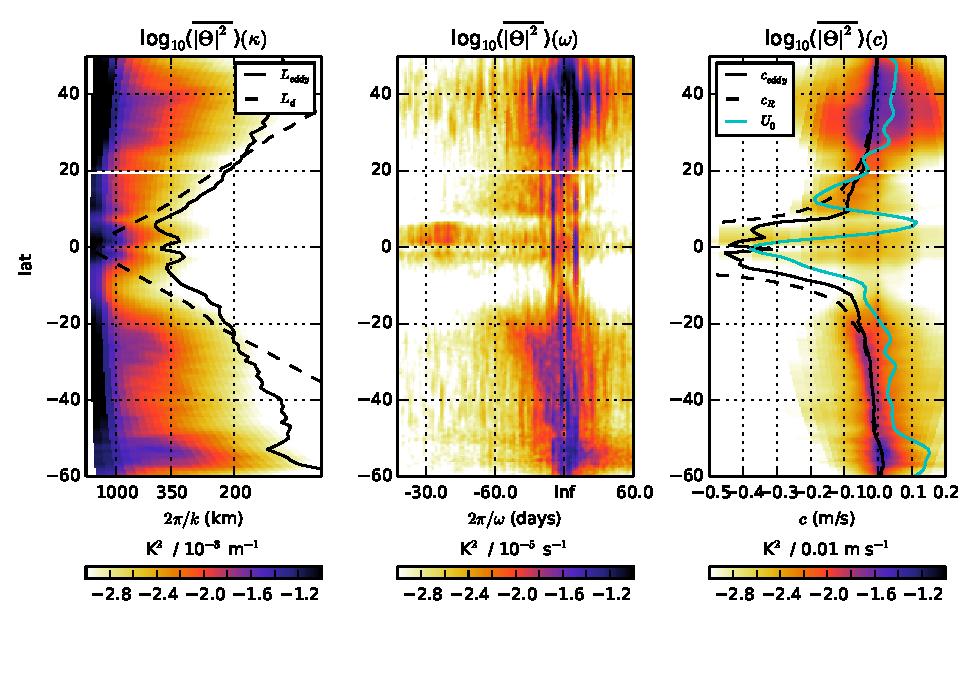
\includegraphics{../figures/50degwide/integrated_spectra_T.pdf}\\
  \caption{Power spectral density of SST variance as a function of latitude and wavenumber (left), frequency (center), and phase speed(right). All color scales are logarithmic. In the left panel, the Rossby deformation radius ($L_d$, from \citealt{TullochEtAl2011}) and the average nonlinear eddy diameter ($L_{eddy}$, from \citealt{CheltonEtAl2011}) are also plotted. In the right panel, the longwave linear Rossby wave phase speed ($c_R$, from \citealt{TullochEtAl2011}), the speed of tracked nonlinear eddies ($c_{eddy}$, from \citealt{CheltonEtAl2011}) and the surface zonal mean flow speed are also plotted.}
  \label{fig:integrated_spectra_T}
\end{figure}

\begin{figure}[t]
  \noindent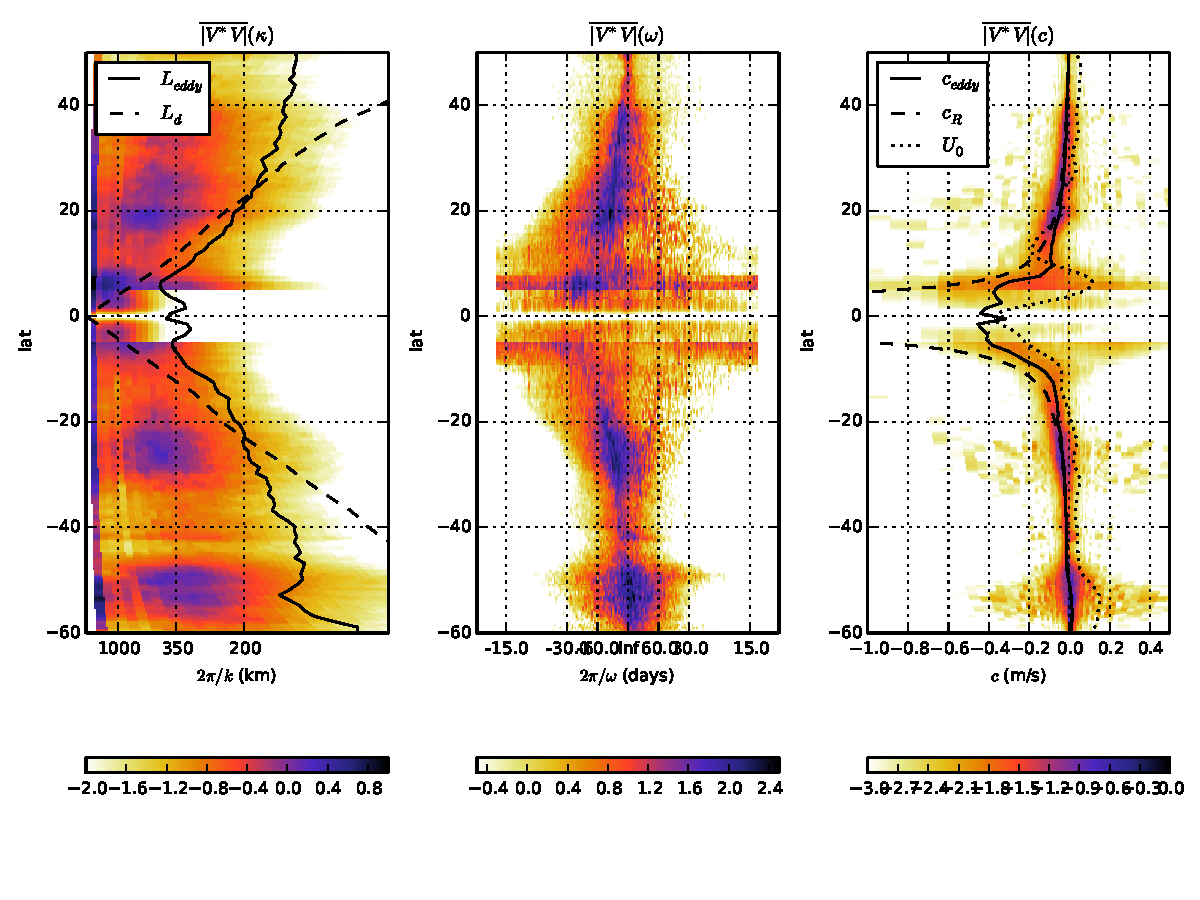
\includegraphics{../figures/50degwide/integrated_spectra_V.pdf}\\
  \caption{The same as Fig.~\ref{fig:integrated_spectra_V}, but for the SSH-derived meridional velocity.}
  \label{fig:integrated_spectra_V}
\end{figure}

\subsection{Eddy Heat Flux Cross Spectra}

Parseval's theorem also applies to the product of $\theta$ and $v$; the eddy heat flux is the same whether expressed as an average of space / time components or a sum of Fourier components. We express this mathematically in our chosen notation as
\begin{equation}
\ol{V\Theta} = \frac{1}{MN} \sum_{m=0}^{M-1} \sum_{n=0}^{N-1} v_{mn} \theta_{mn} = \sum_{j=-\frac{M}{2}}^{\frac{M}{2}-1} \sum_{k=0}^{\frac{N}{2}-1} \Re \{ V_{jk}^\ast  \Theta_{jk} \} \ .
\end{equation}
Just as described above, we can sum the components of $\Re \{ V_{jk}^\ast  \Theta_{jk} \}$ selectively to define $\ol{V\Theta}(\varphi, \kappa)$, $\ol{V\Theta}(\varphi, \omega)$, and $\ol{V\Theta}(\varphi, c)$. These functions are plotted in  Fig.~\ref{fig:integrated_spectra_VT}. Unlike the power spectra described above $\ol{V\Theta}$ can take both positive and negative values, corresponding to northward and southward heat transport. As seen in Fig.~\ref{fig:integrated_spectra_VT}, the eddy heat flux is poleward in both hemispheres, except near the equator, where it reverses. This is consistent with the mean SST gradient, which also reverses near the equator; the eddy flux is always down gradient. (The eddy diffusivity is discussed in Sec.~5).

The spatial structure of the magnitude of the three $\ol{V\Theta}$ functions resembles that of $\ol{|V|^2}$ more than it does that of $\ol{|\Theta|^2}$. While $\ol{|\Theta|^2}(\kappa)$ peaks at the lowest wavenumbers at every latitude, both  $\ol{|V|^2}(\kappa)$ and $\ol{V\Theta}(\kappa)$ peak at an intermediate wavenumber, presumably one associated with mesoscale eddies.

\begin{figure}[t]
  \noindent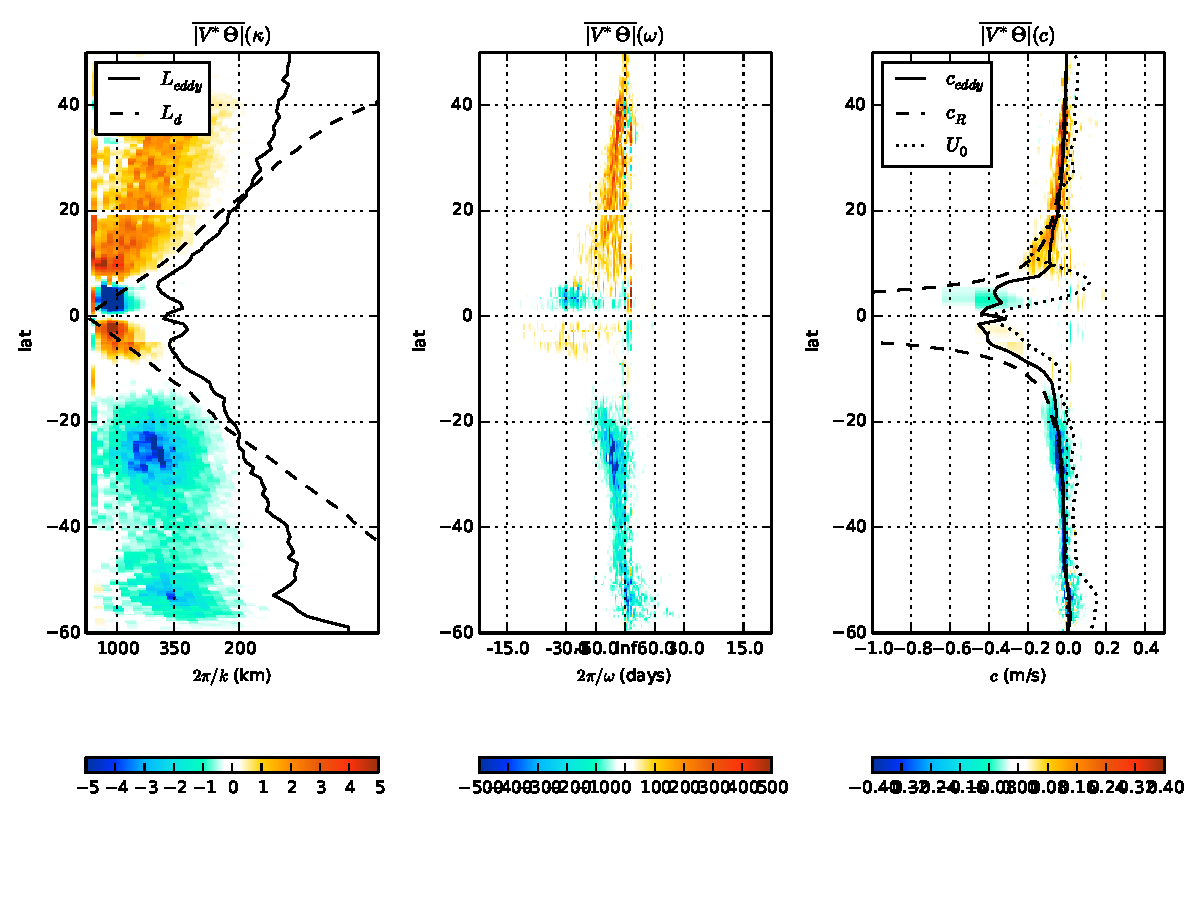
\includegraphics{../figures/50degwide/integrated_spectra_VT.pdf}\\
  \caption{The same as Fig.~\ref{fig:integrated_spectra_V}, but for the heat flux cross-specta.}
  \label{fig:integrated_spectra_VT}
\end{figure}


\section{Wavenumber, Frequency and Phase Speed Spectra}

\section{Discussion and Conclusions}
Atmospheric waves propagate meridionally, but this propagation is constrained by their phase speed: they break when they encounter ``critical latitudes'' at which their phase speed matches the background mean flow. These dynamics leave a clear signature in atmospheric phase-speed cospecta \citep{ChenHeld2007}. Ocean eddies, in contrast, do not propagate far in latitude. However, we argue that the phase phase speed is still an important factor in understanding ocean eddy fluxes, since it plays a significant role in determining the eddy diffusivity \citep{AbernatheyEtAl2010,FerrariNikurashin2010}. In this study we show that the surface eddy heat flux at each latitude is relatively concentrated around the long-wave Rossby wave phase speed.


% a low frequency cutoff doesn't necessarily filter out non-mesoscale motions. Consider a stationary eddy in the ACC, propagating upstream but locked in place

\begin{figure*}[t!]
  \noindent %\includegraphics{theta_spinup_new.pdf}\\
  \caption{Blah.}
  \label{fig:a}
\end{figure*}

% Use appendix}[A], {appendix}[B], etc. etc. in place of appendix if you have multiple appendixes.
\ifthenelse{\boolean{dc}}
{}
{\clearpage}

% Create a bibliography directory and place your .bib file there.
% -REMOVE ALL DIRECTORY PATHS TO REFERENCE FILES BEFORE SUBMITTING TO THE AMS FOR PEER REVIEW
\ifthenelse{\boolean{dc}}
{}
{\clearpage}
\bibliographystyle{ametsoc}
\bibliography{../bibliography/references}

%%%%%%%%%%%%%%%%%%%%%%%%%%%%%%%%%%%%%%%%%%%%%%%%%%%%%%%%%%%%%%%%%%%%%
% FIGURES-REMOVE ALL DIRECTORY PATHS TO FIGURE FILES BEFORE SUBMITTING TO THE AMS FOR PEER REVIEW
%%%%%%%%%%%%%%%%%%%%%%%%%%%%%%%%%%%%%%%%%%%%%%%%%%%%%%%%%%%%%%%%%%%%%
%\begin{figure}[t]
%  \noindent\includegraphics[width=19pc,angle=0]{figure01.pdf}\\
%  \caption{Enter the caption for your figure here.  Repeat as
%  necessary for each of your figures. Figure from \protect\cite{Knutti2008}.}\label{f1}
%\end{figure}
%%%%%%%%%%%%%%%%%%%%%%%%%%%%%%%%%%%%%%%%%%%%%%%%%%%%%%%%%%%%%%%%%%%%%
% TABLES
%%%%%%%%%%%%%%%%%%%%%%%%%%%%%%%%%%%%%%%%%%%%%%%%%%%%%%%%%%%%%%%%%%%%%
%\begin{table}[t]
%\caption{This is a sample table caption and table layout.  Enter as many tables as
%  necessary at the end of your manuscript. Table from Lorenz (1963).}\label{t1}
%\begin{center}
%\begin{tabular}{ccccrrcrc}
%\hline\hline
%$N$ & $X$ & $Y$ & $Z$\\
%\hline
% 0000 & 0000 & 0010 & 0000 \\
% 0005 & 0004 & 0012 & 0000 \\
% 0010 & 0009 & 0020 & 0000 \\
% 0015 & 0016 & 0036 & 0002 \\
% 0020 & 0030 & 0066 & 0007 \\
% 0025 & 0054 & 0115 & 0024 \\
%\hline
%\end{tabular}
%\end{center}
%\end{table}
%
\end{document}
